\documentclass{standalone}
\usepackage{tikz}
\usepackage{verbatim}
\usetikzlibrary{positioning}
\begin{document}
\pagestyle{empty}
  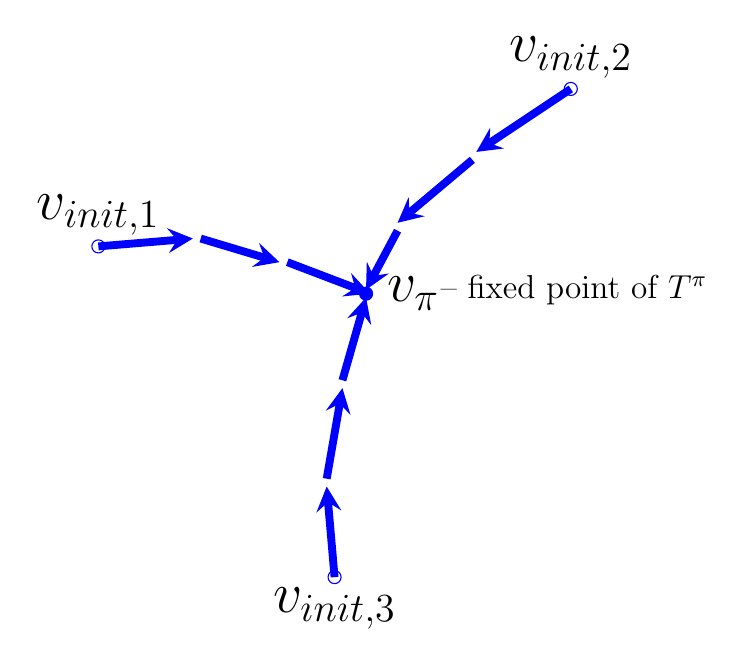
\begin{tikzpicture}
  	\node[draw,circle,scale=1/2,blue] at (-4, 0.6) {};
  	\node at (-4, 1) {\huge $v_{init, 1}$};
  	\node[draw,circle,scale=1/2,blue] at (2, 2.6) {};
  	\node at (2, 3) {\huge $v_{init, 2}$};
  	\node[draw,circle,scale=1/2,blue] at (-1, -3.6) {};
  	\node at (-1, -4) {\huge $v_{init, 3}$};
  	\node[draw, fill, circle,scale=1/2,blue] at (-0.6, 0.) {};
  	\node at (0, 0) {\huge $v_\pi$};
  	\node at (2.04, 0.04) {\large -- fixed point of $T^\pi$};
  	\draw[-stealth, blue, line width=1 mm] (-4, 0.6) -- (-2.8, 0.7);
  	\draw[-stealth, blue, line width=1 mm] (-2.7, 0.7) -- (-1.7, 0.4);
  	\draw[-stealth, blue, line width=1 mm] (-1.6, 0.4) -- (-0.55, 0.);
  	
  	\draw[-stealth, blue, line width=1 mm] (2, 2.6) -- (0.8, 1.8);
  	\draw[-stealth, blue, line width=1 mm] (0.75, 1.7) -- (-0.2, 0.9);
  	\draw[-stealth, blue, line width=1 mm] (-0.2, 0.8) -- (-0.6, 0.05);
  	
  	\draw[-stealth, blue, line width=1 mm] (-1, -3.6) -- (-1.1, -2.45);
  	\draw[-stealth, blue, line width=1 mm] (-1.1, -2.35) -- (-0.9, -1.2);
  	\draw[-stealth, blue, line width=1 mm] (-0.9, -1.1) -- (-0.6, -0.05);

  \end{tikzpicture}
\end{document}